\section{Thực hiện mạch đo nhiệt độ}

\subsection{Mô phỏng trên Multisim}
\begin{figure}[H]
	\centering
	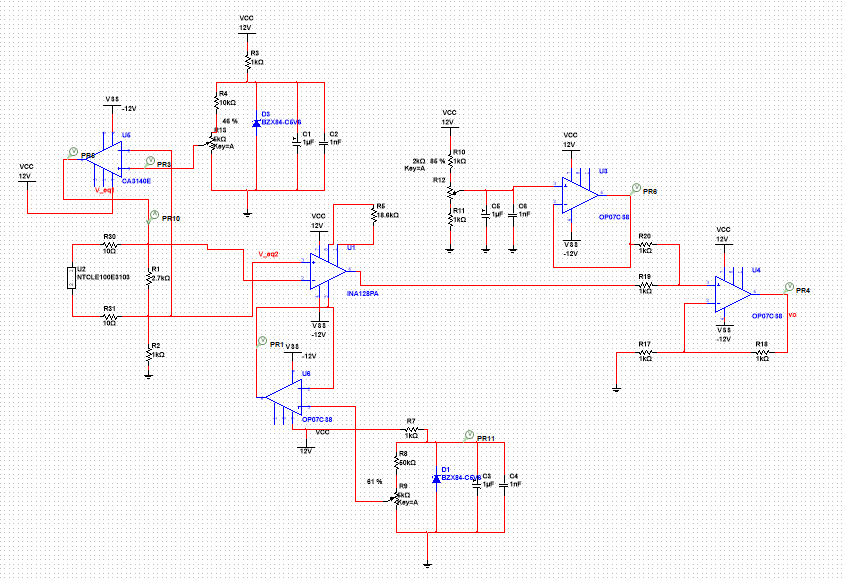
\includegraphics[width=0.7\linewidth]{my-chapters/my-images/Circuit_sim/overview_mul}
	\caption{Schematic Nmultisim}
	\label{fig:overviewmul}
\end{figure}

\begin{itemize}[label=-]
	\item Để tạo các điện áp tham chiếu 1V và 0.2V nhóm sử dụng diode zenner BZX84C5V6 có điện áp ngược ổn định 5.6V.
	\item Bỏ bớt 1 opamp giữa INA128 (U1) và ) OP7CS8 ( U4) có vai trò như 1 bộ đệm vì điều này ko cần thiết tốn tài nguyên.
\end{itemize}

\begin{figure}[H]
	\centering
	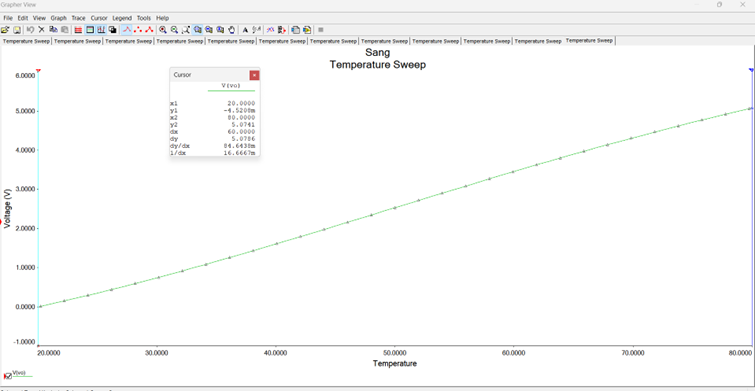
\includegraphics[width=0.7\linewidth]{my-chapters/my-images/Circuit_sim/sim_multisim}
	\caption{Mô phỏng trên Multisim}
	\label{fig:simmultisim}
\end{figure}

\subsection{Thực thi mạch trên Altium}

\subsubsection{Schematic}

\begin{figure}[H]
	\centering
	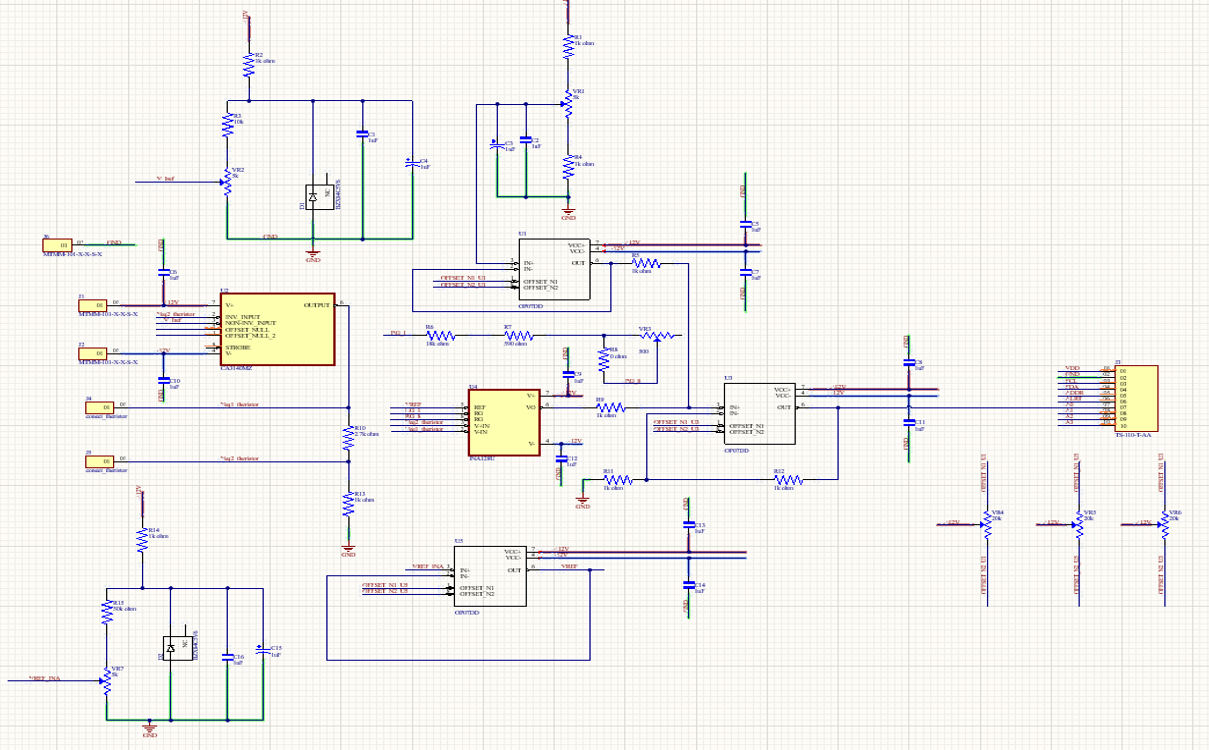
\includegraphics[width=0.8\linewidth]{my-chapters/my-images/Circuit_sim/PCB_schematic_sensor}
	\caption{Schematic của Mạch đọc nhiệt độ.}
	\label{fig:pcbschematicsensor}
\end{figure}

\subsubsection{Layout}

\begin{figure}[H]
	\centering
	\begin{minipage}{.45\linewidth}
		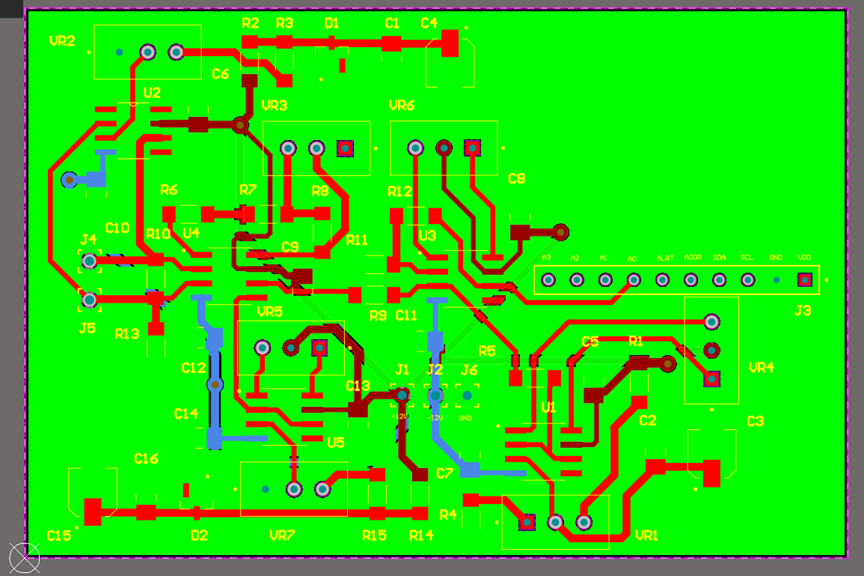
\includegraphics[width=\linewidth]{my-chapters/my-images/Circuit_sim/PCB_layout_sensor}
	\end{minipage}
	\begin{minipage}{.45\linewidth}
		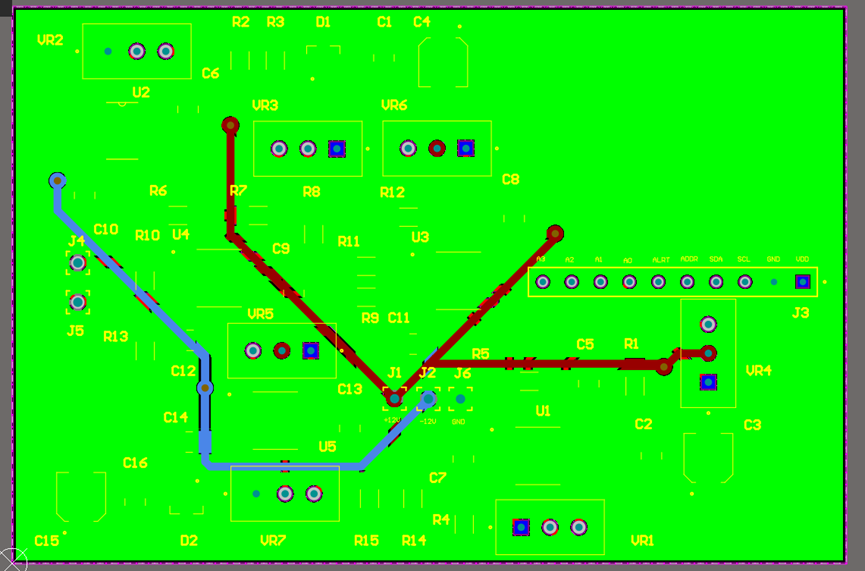
\includegraphics[width=\linewidth]{my-chapters/my-images/Circuit_sim/PCB_layout_sensor_1}
	\end{minipage}
	\caption{Layout của Mạch đọc nhiệt độ.}
	\label{fig:pcblayoutsensor}
\end{figure}

\begin{figure}[H]
	\centering
	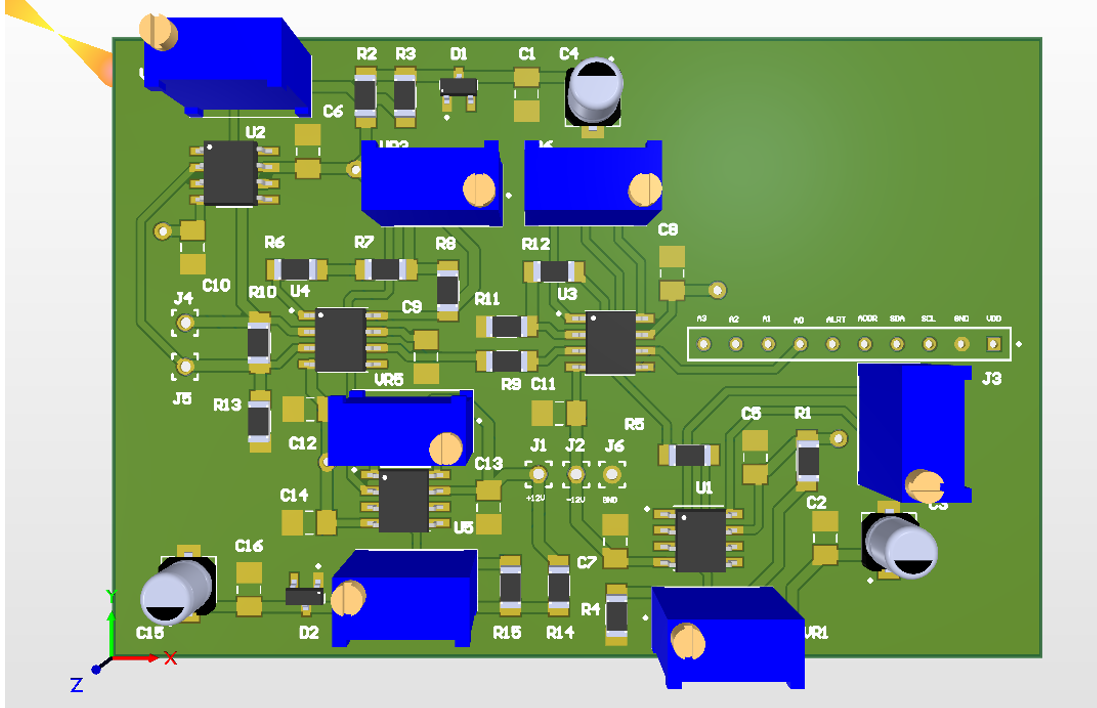
\includegraphics[width=0.7\linewidth]{my-chapters/my-images/Circuit_sim/PCB_3d}
	\caption{Mô hình 3D của Mạch đọc nhiệt độ.}
	\label{fig:pcb3d}
\end{figure}

\begin{figure}[H]
	\centering
	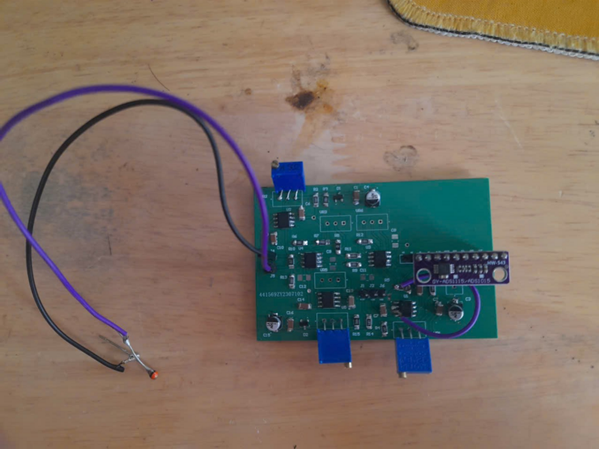
\includegraphics[width=0.7\linewidth]{my-chapters/my-images/Circuit_sim/PCB_thucte}
	\caption{Mạch thực tế của Mạch đọc nhiệt độ.}
	\label{fig:pcbthucte}
\end{figure}

\subsubsection{Thực hiện test mạch thực tế}

\begin{figure}[H]
	\centering
	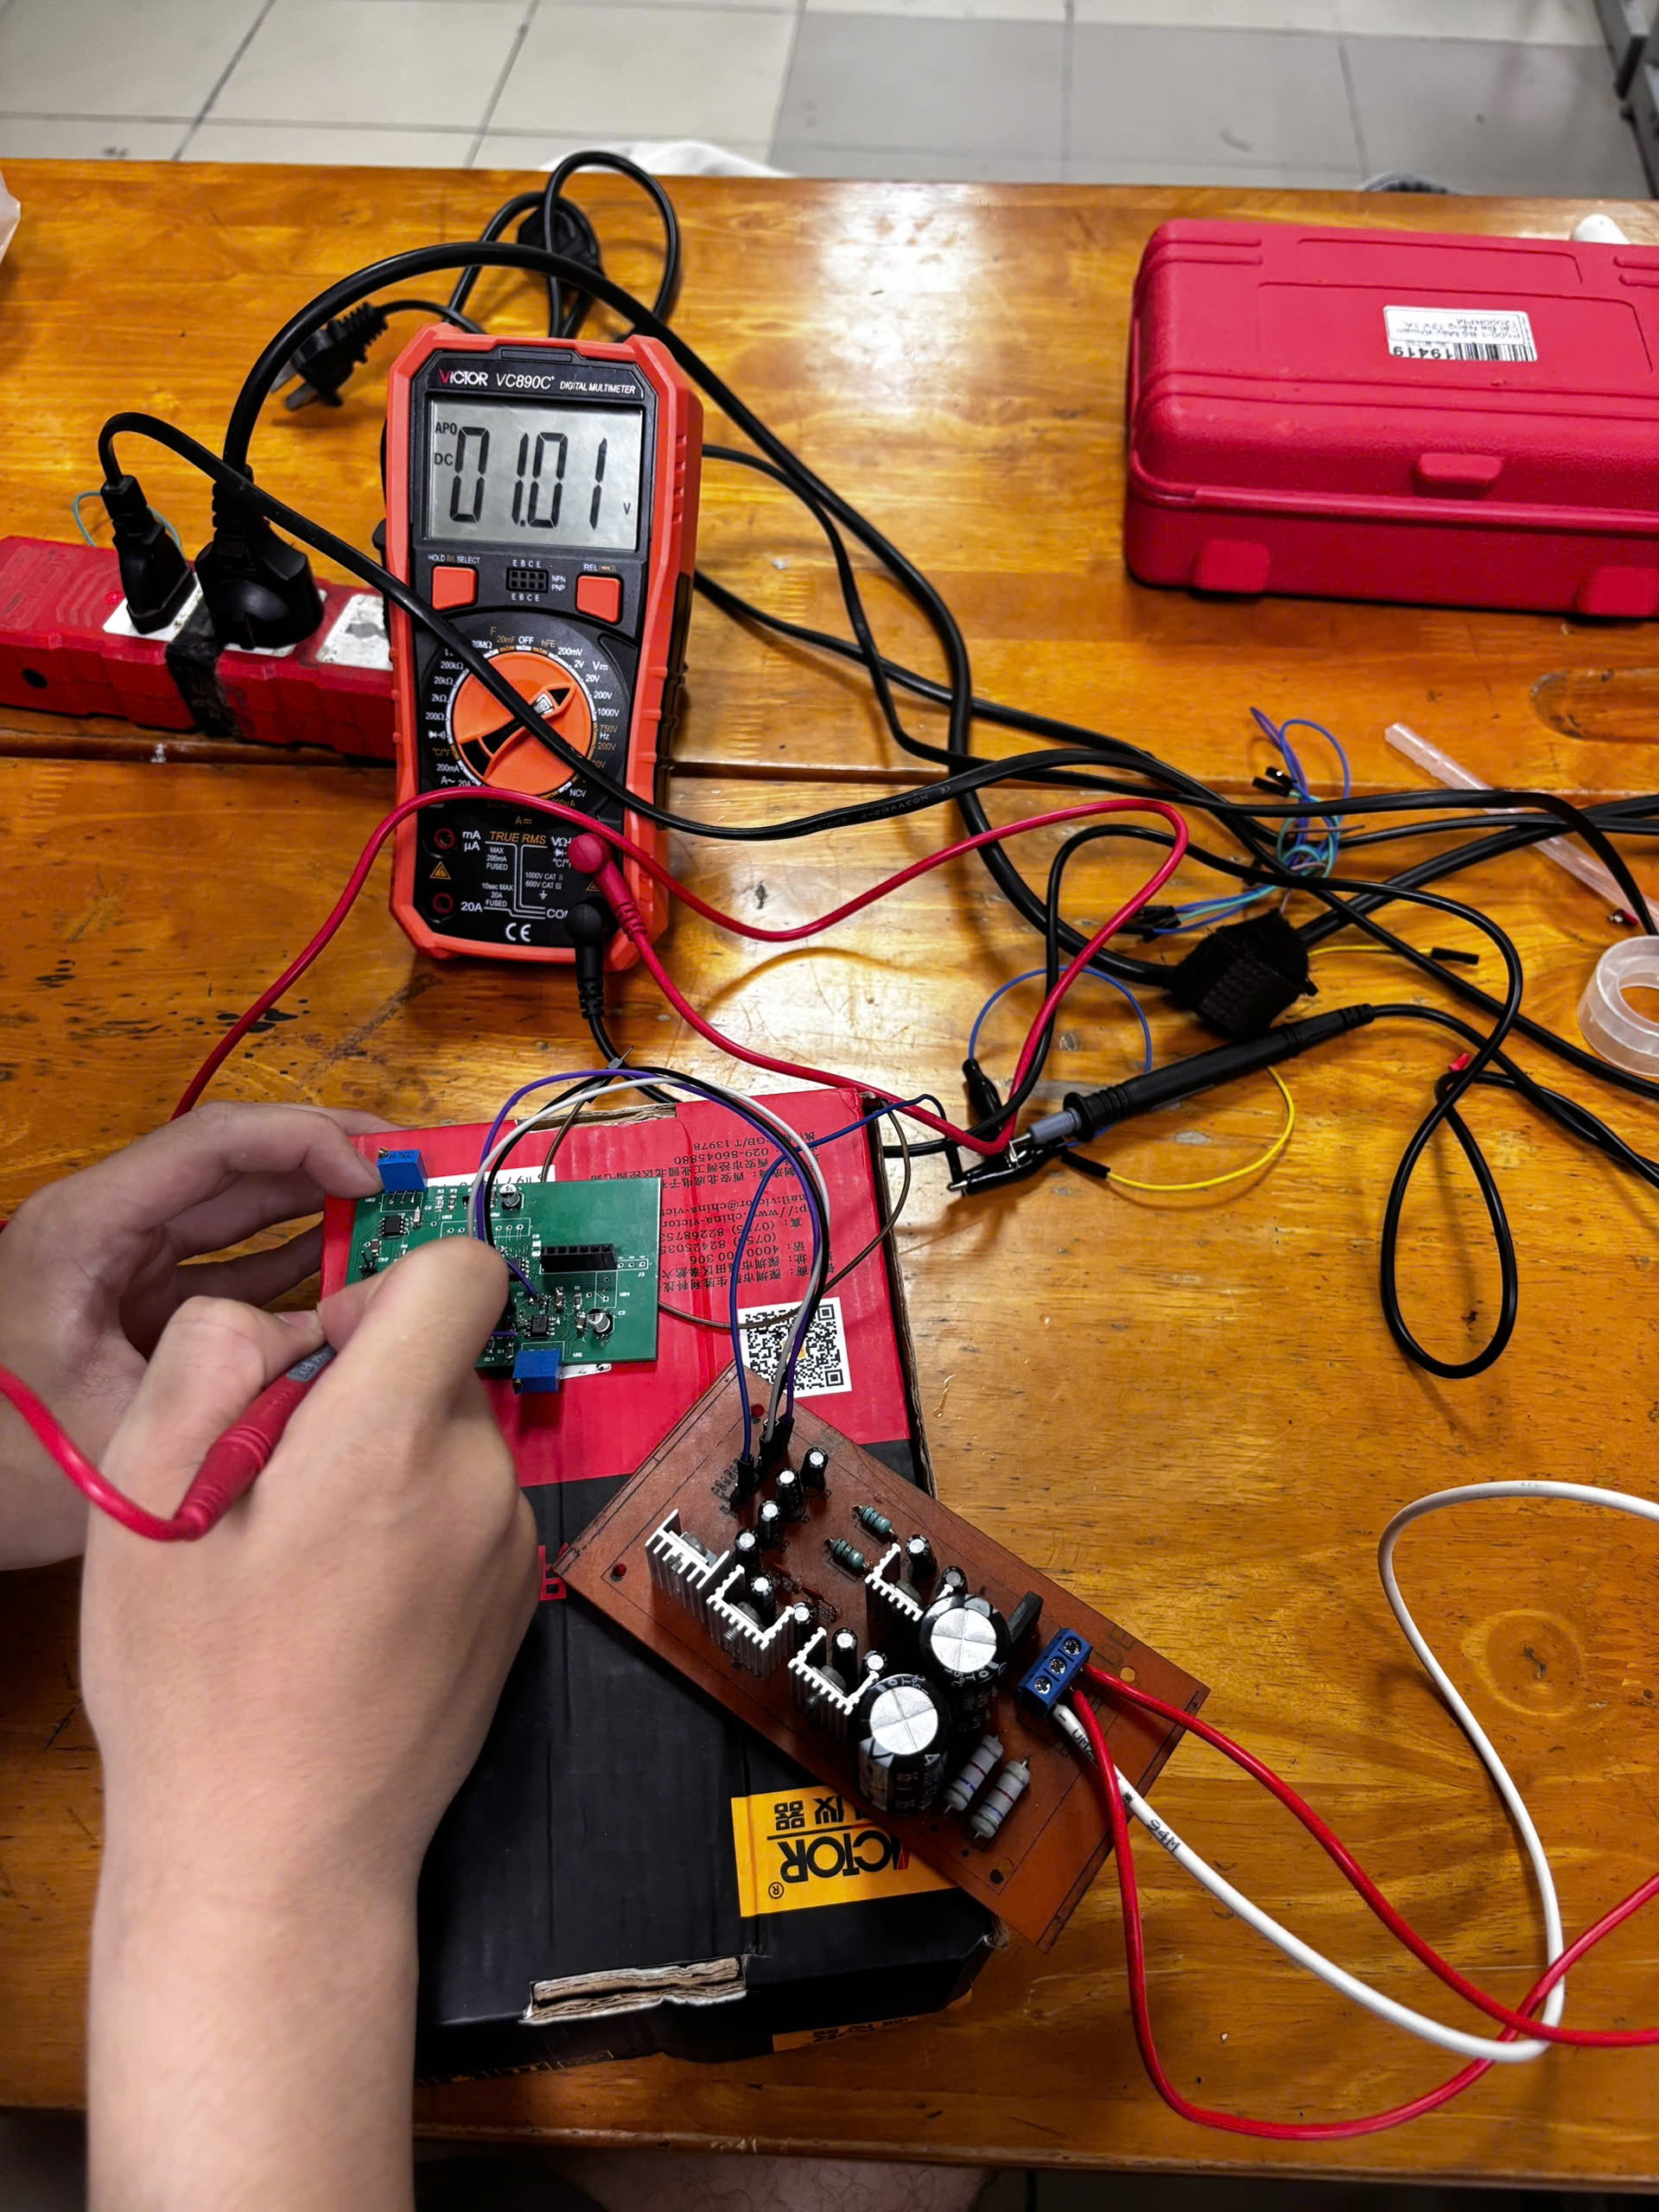
\includegraphics[width=0.7\linewidth]{my-chapters/my-images/Circuit_sim/CIRCUIT_1mA}
	\caption{Kiểm tra tạo nguồn dòng $1m\textsf{A}$.}
	\label{fig:circuit1ma}
\end{figure}

Ta thấy mạch đã tạo điện áp 1V ngay trên điện trở $1\textsf{K}\Omega$:

\begin{figure}[H]
	\centering
	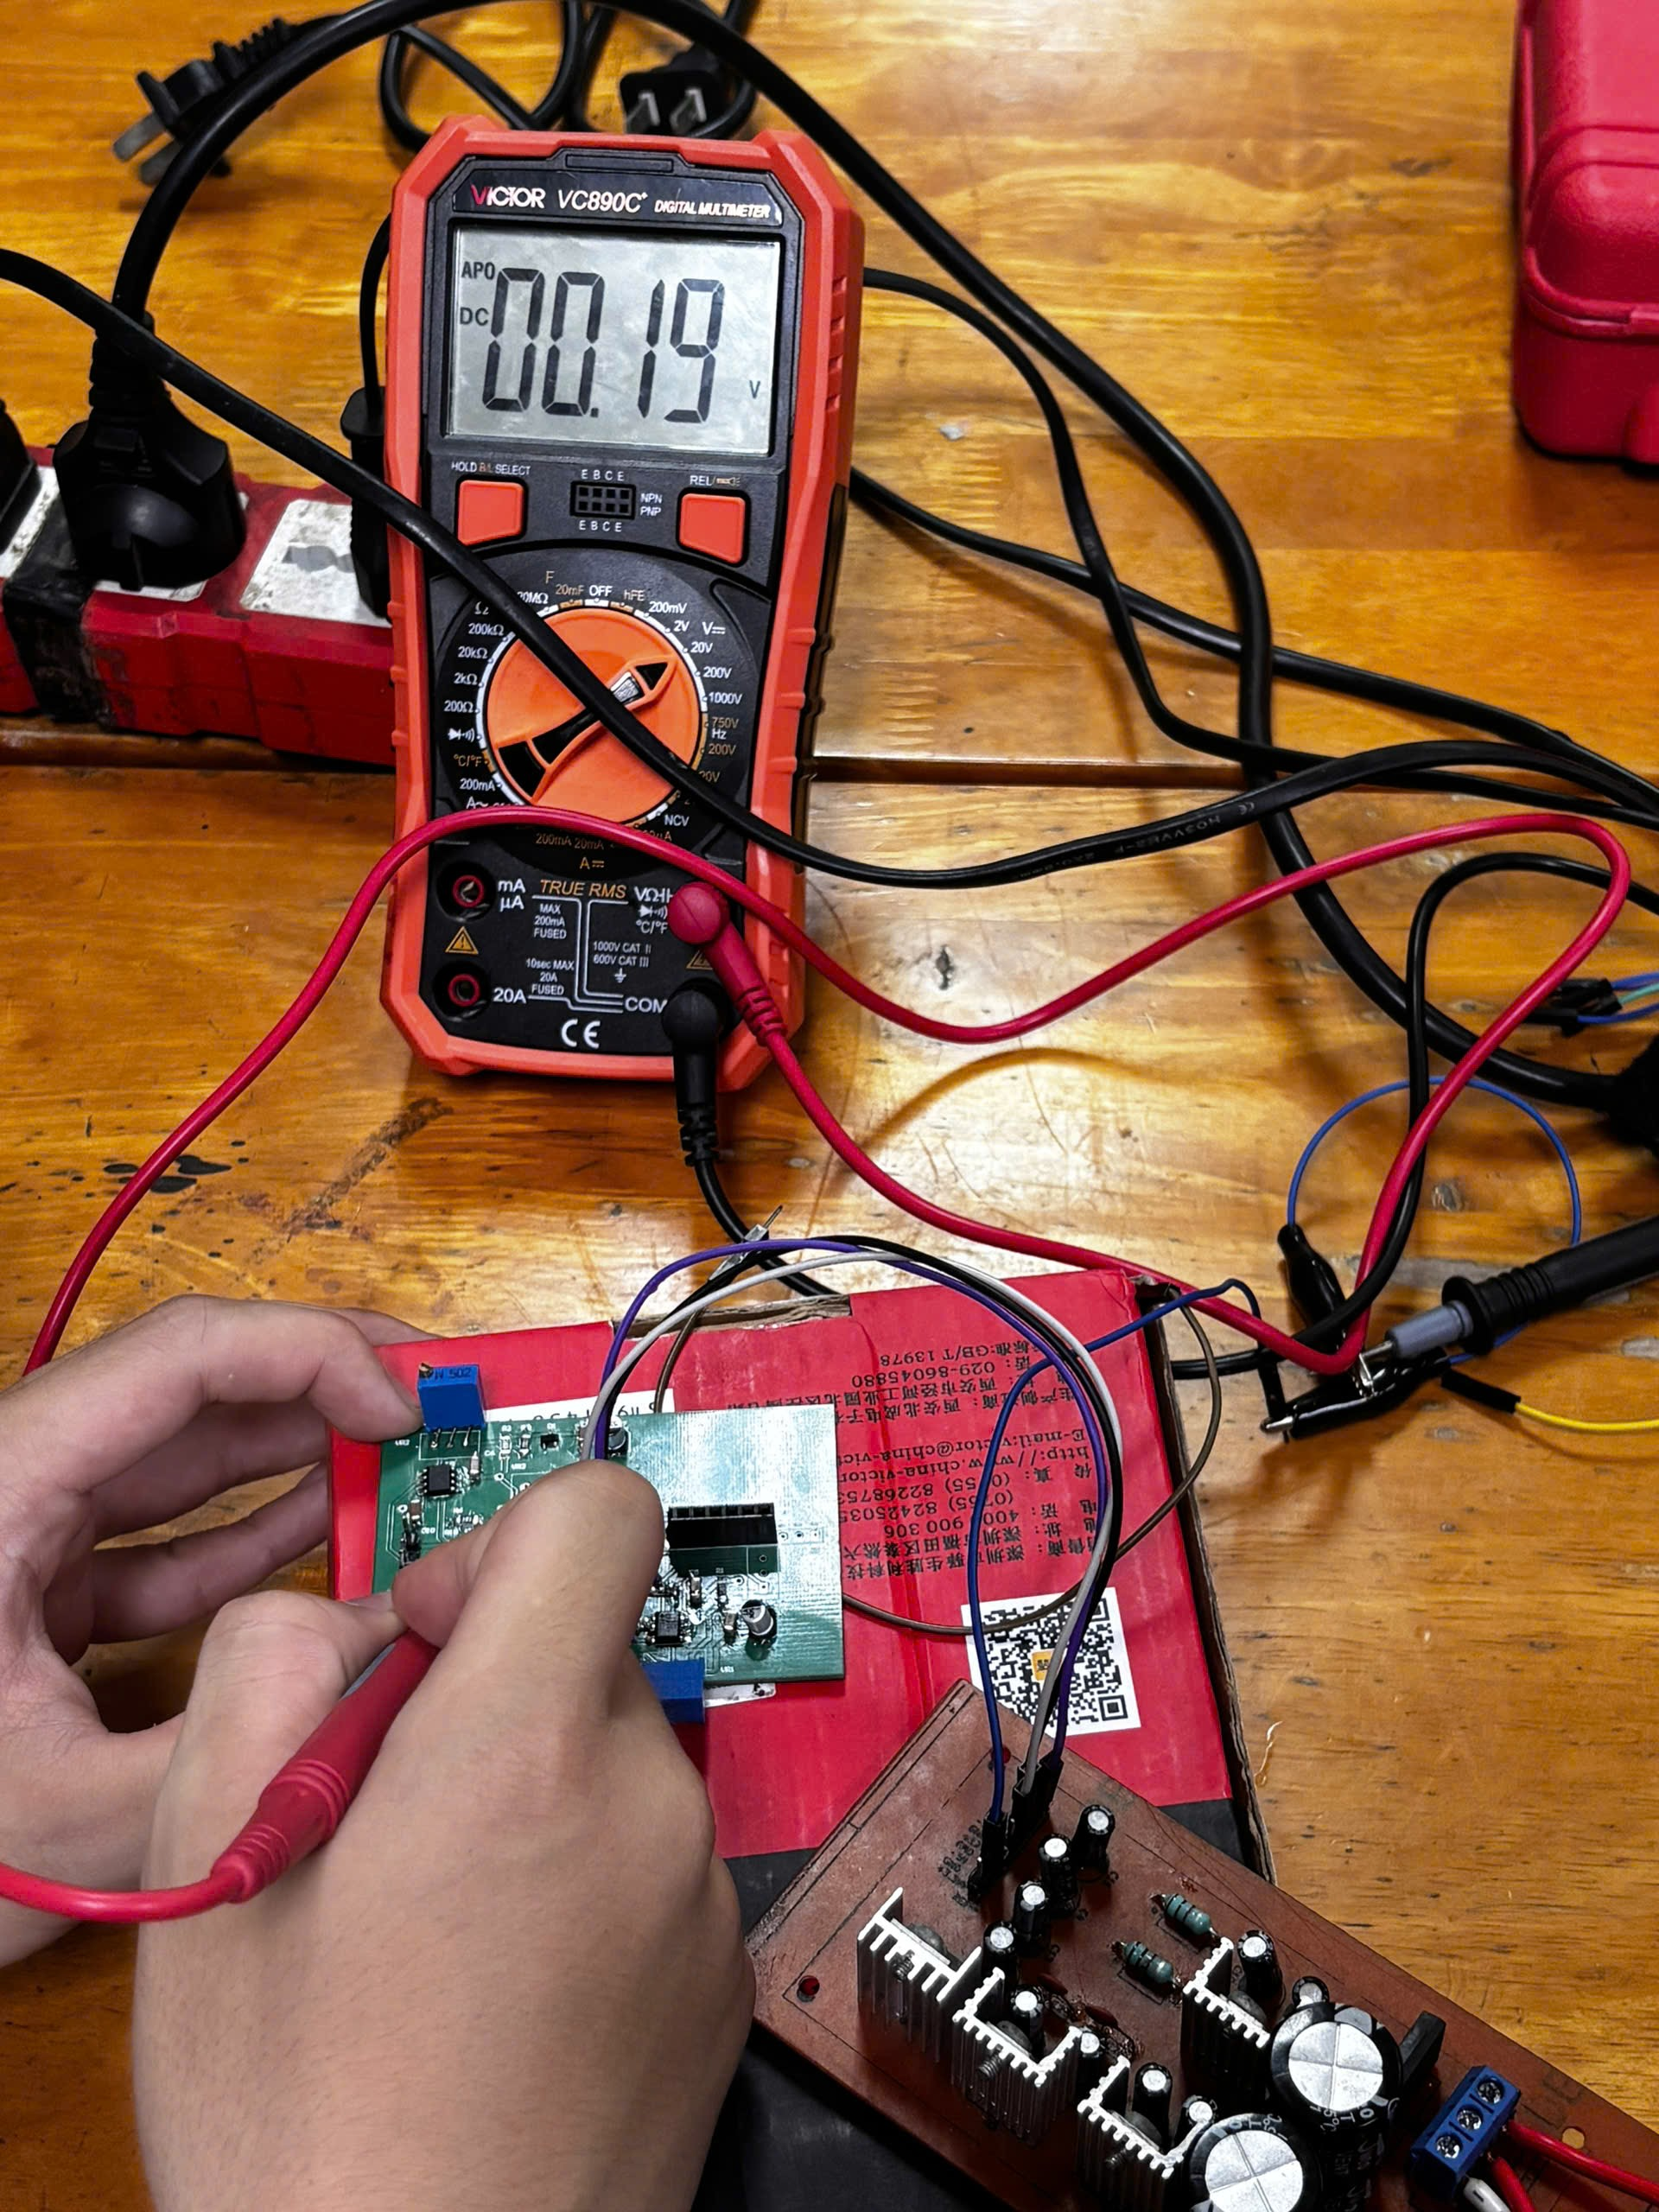
\includegraphics[width=0.7\linewidth]{my-chapters/my-images/Circuit_sim/CIRCUIT_0_2V}
	\caption{Kiểm tra mạch tao điện áp tham chiếu cho INA128 Theo lý thuyết là $0.2\textsf{V}$.}
	\label{fig:circuit02v}
\end{figure}

\begin{figure}[H]
	\centering
	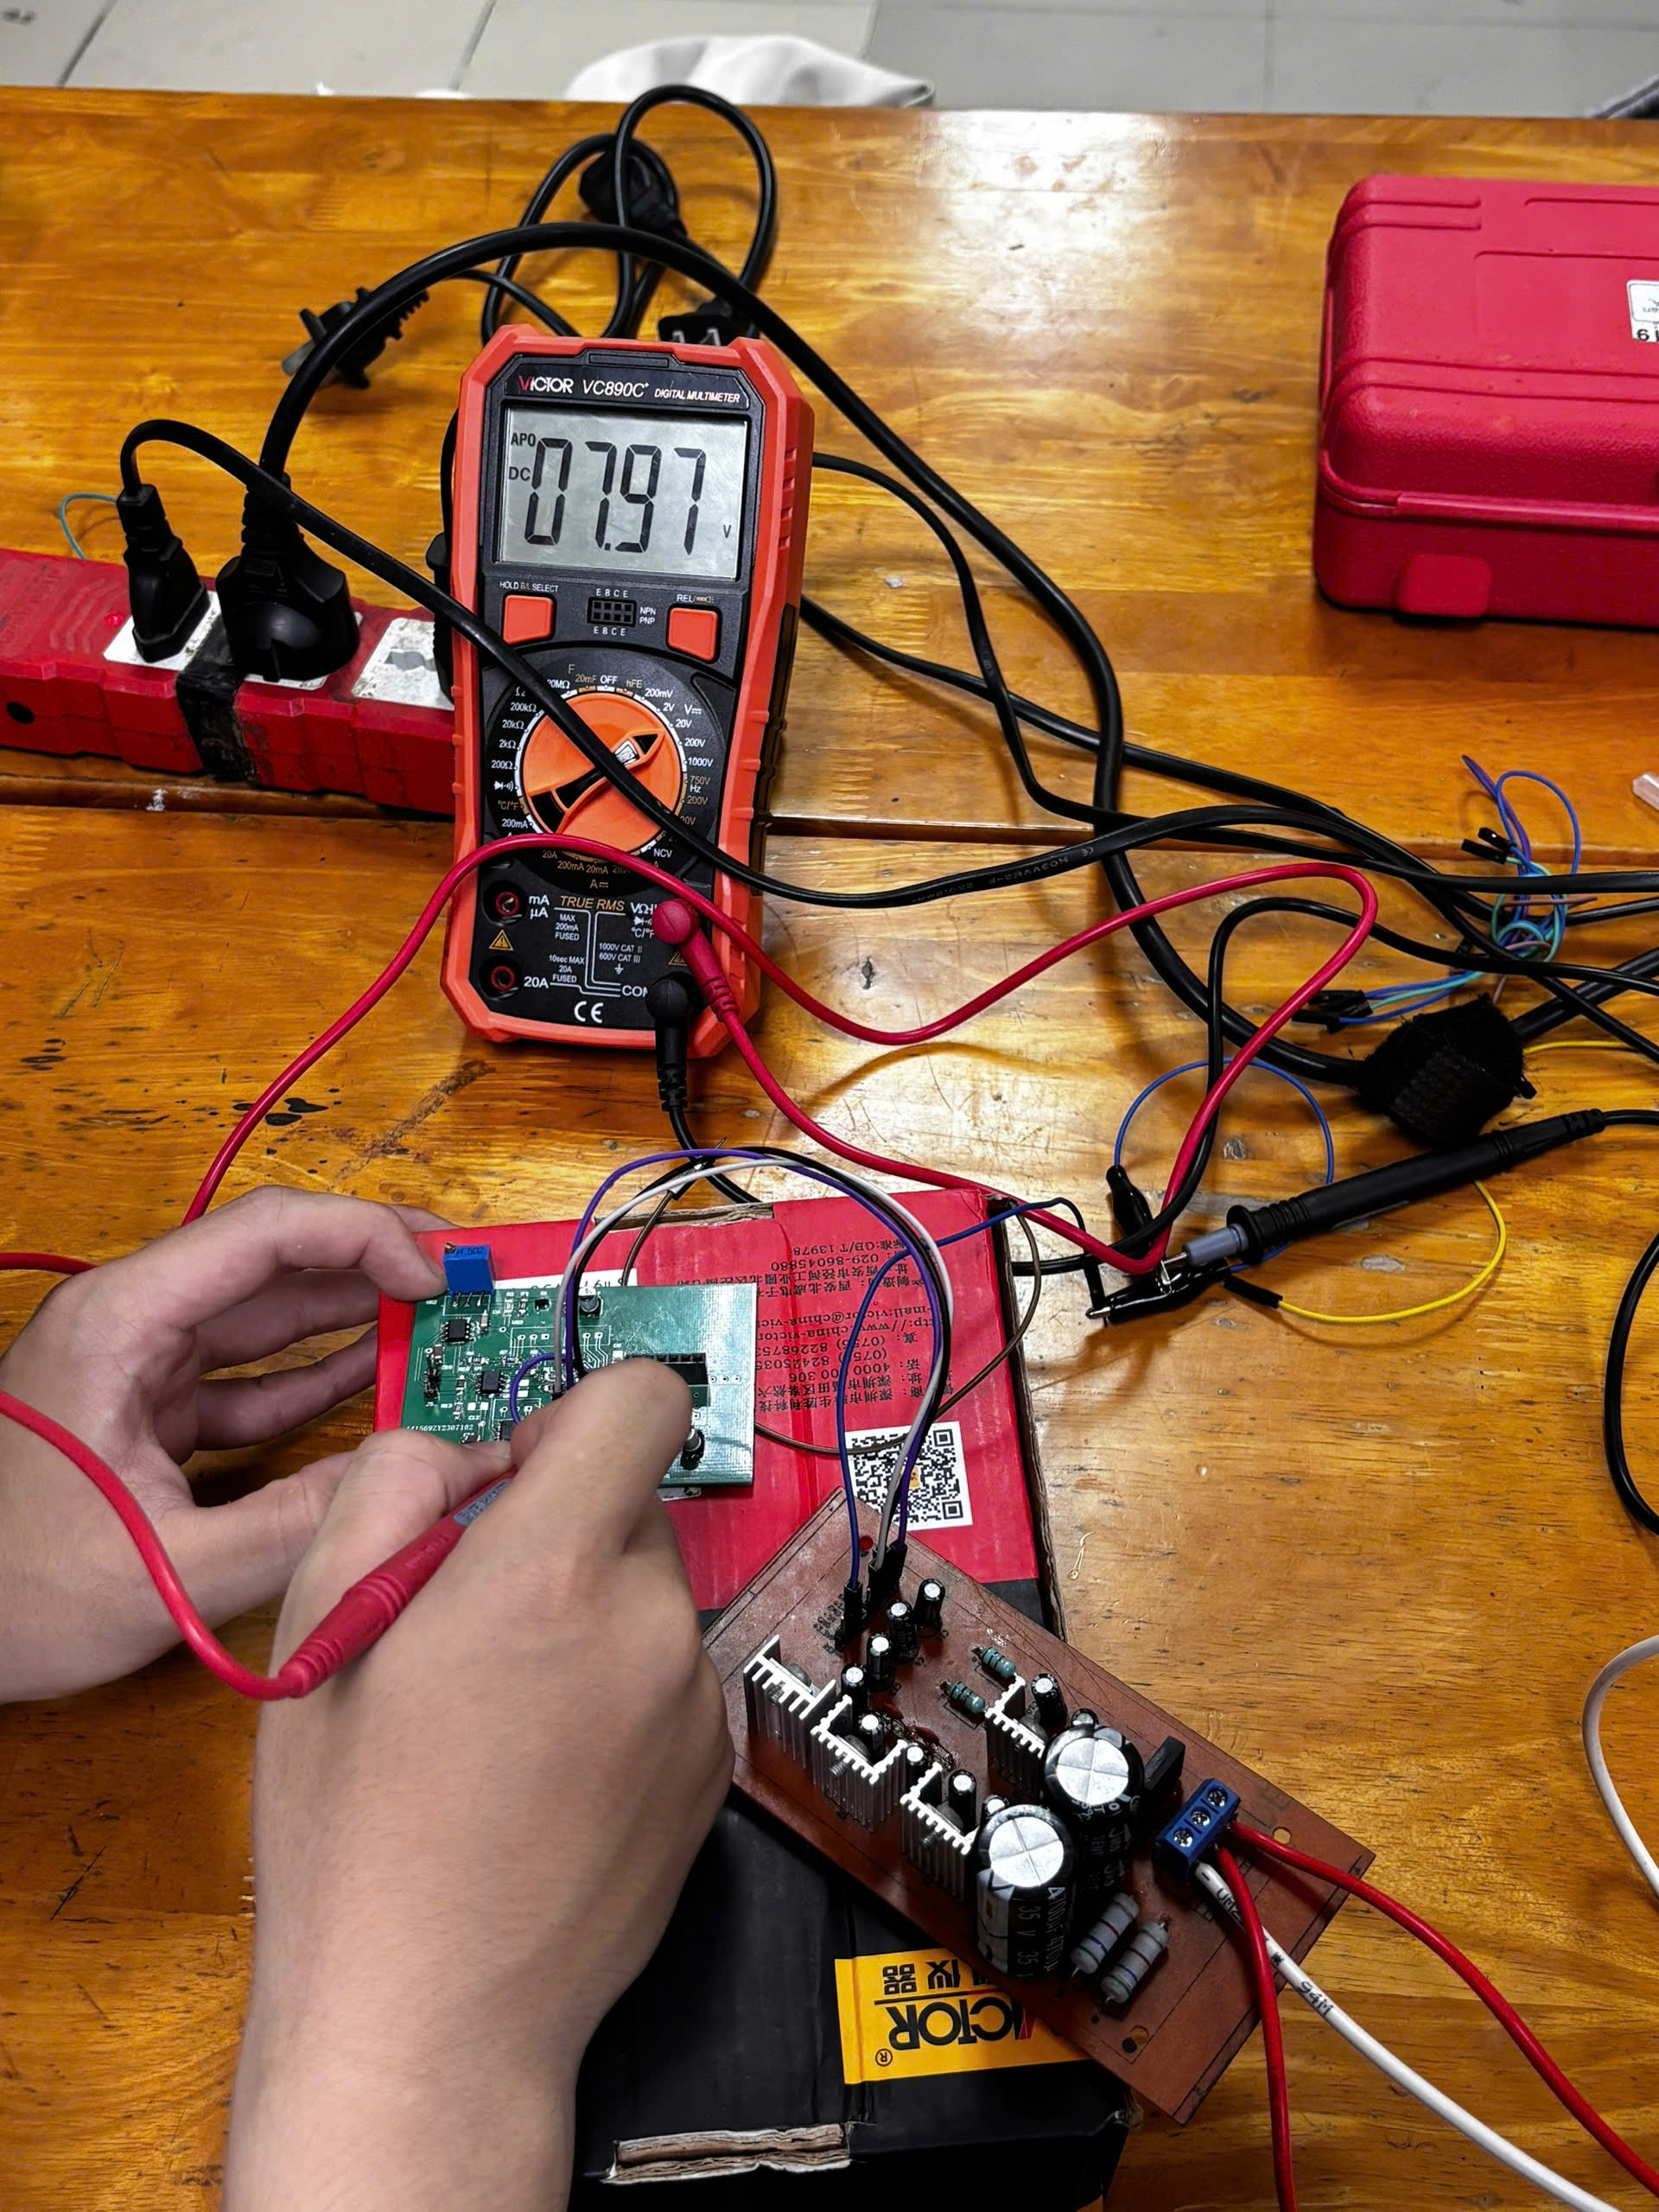
\includegraphics[width=0.7\linewidth]{my-chapters/my-images/Circuit_sim/CIRCUIT_8V}
	\caption{Kiểm tra mạch tạo điên áp cộng $8\textsf{V}$.}
	\label{fig:circuit8v}
\end{figure}

\begin{figure}[H]
	\centering
	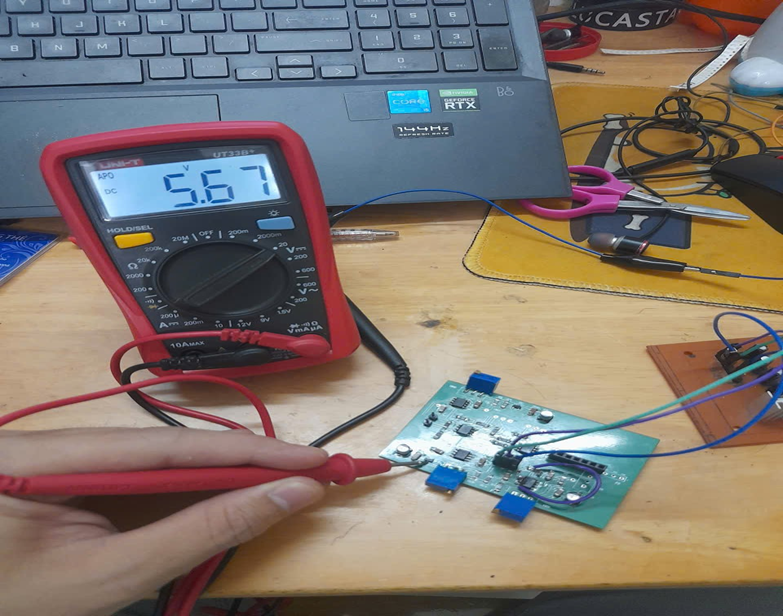
\includegraphics[width=0.7\linewidth]{my-chapters/my-images/Circuit_sim/CIRCUIT_check_zenor}
	\caption{Kiểm tra điện áp Zenner.}
	\label{fig:circuitcheckzenor}
\end{figure}

Nhóm tiến hành đo đạc lần 1 và 2 và kết quả thu được khi chưa calibre mạch (video khảo sát lần 1 :\href{https://youtu.be/ByMETPjAgkQ}{thislink}) ; (video khảo sát lần 2 : \href{https://youtu.be/FqDw9E245dE}{thislink})

\begin{table}[H]
	\centering
	\caption{Bảng số liệu đo đạc điện áp theo nhiệt độ}
	\vspace{0.2cm}
	\begin{tabular}{|c|c|c|}
		\hline
		\textbf{Nhiệt độ} & \textbf{Lần 1 (V)} & \textbf{Lần 2 (V)} \\
		\hline
		15$^\circ$C & 0.45 & 0.42 \\
		\hline
		20$^\circ$C & 0.72 & 0.57 \\
		\hline
		25$^\circ$C & 0.88 & 0.88 \\
		\hline
		30$^\circ$C & 1.16 & 1.13 \\
		\hline
		35$^\circ$C & 1.4 & 1.09 \\
		\hline
		40$^\circ$C & 1.72 & 1.84 \\
		\hline
		45$^\circ$C & 2.03 & 2.17 \\
		\hline
		50$^\circ$C & 2.38 & 2.43 \\
		\hline
		55$^\circ$C & 2.77 & 2.75 \\
		\hline
		60$^\circ$C & 3.13 & 3.08 \\
		\hline
		65$^\circ$C & 3.51 & 3.77 \\
		\hline
		70$^\circ$C & 5.7 & 9.16 \\
		\hline
		75$^\circ$C & 9.29 & 8.9 \\
		\hline
		80$^\circ$C & 9.16 & 8.67 \\
		\hline
	\end{tabular}
\end{table}

\begin{itemize}
	\item \textbf{Nhận xét:} Điện áp có xu hướng tăng theo nhiệt độ nhưng từ khoảng 65 độ trở đi điện áp đạt tới 8 đến 9V.
\end{itemize}

Nhóm tiến hành calibre mạch đầu tiên nhóm đo điện trở ban đầu của NTC và kết quả đo là $8.08 \, k\Omega$ từ phương trình trong datasheet ta có:

\[
\text{Với } Ref = 10k, \quad T = 303.7 \, K, \quad t = 30 (^\circ C)
\]

Nhưng khi đo đạc điện áp ở ngõ ra ban đầu là $1.5V$ điều này cho thấy sự sai lệch khá lớn với lý thuyết khi tại $30 (^\circ C)$ điện áp tại ngõ ra sẽ khoảng $0.738 \, V$, độ lệch khoảng $0.762 \, V$. Chính vì vậy nhóm tiến hành tinh chỉnh điện áp cộng ở ngõ ra $8V$ giảm đi một lượng xấp xỉ $0.762V$ thành $7.25 \, V$.

\begin{figure}[H]
	\centering
	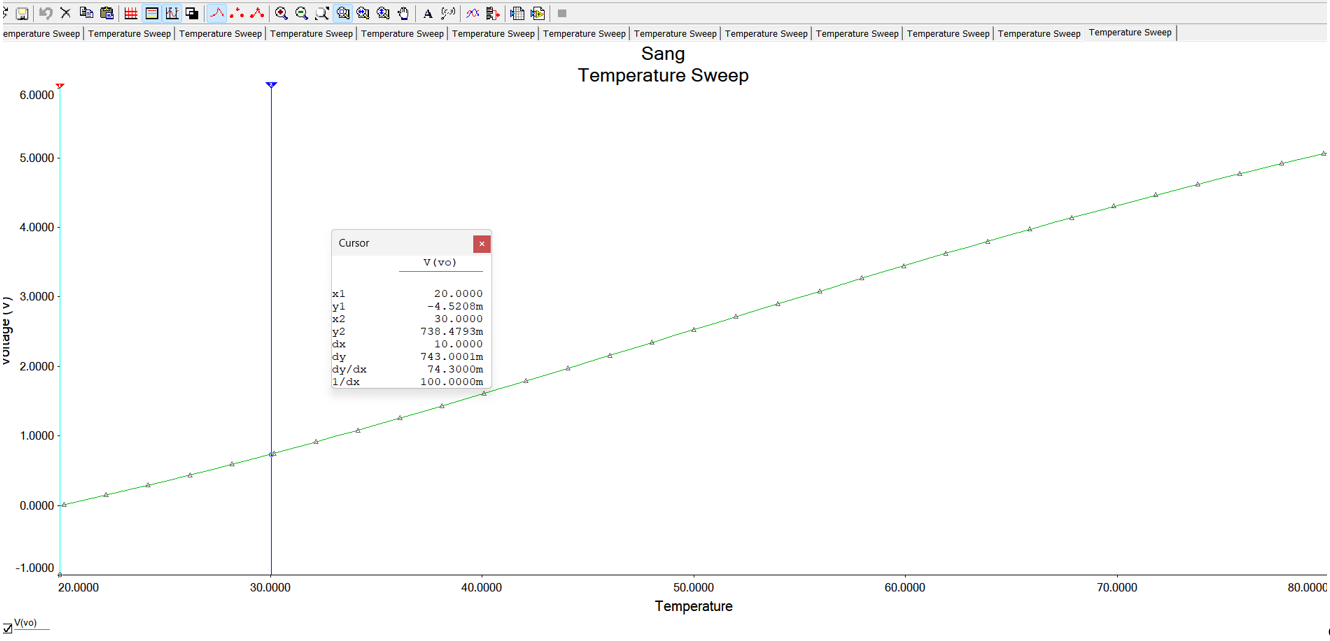
\includegraphics[width=0.9\linewidth]{my-chapters/my-images/Circuit_sim/CIRCUIT_pre_check}
	\caption{Điện áp ngõ ra tại $30^{o}C$ theo lý thuyết.}
	\label{fig:circuitprecheck}
\end{figure}

\begin{figure}[H]
	\centering
	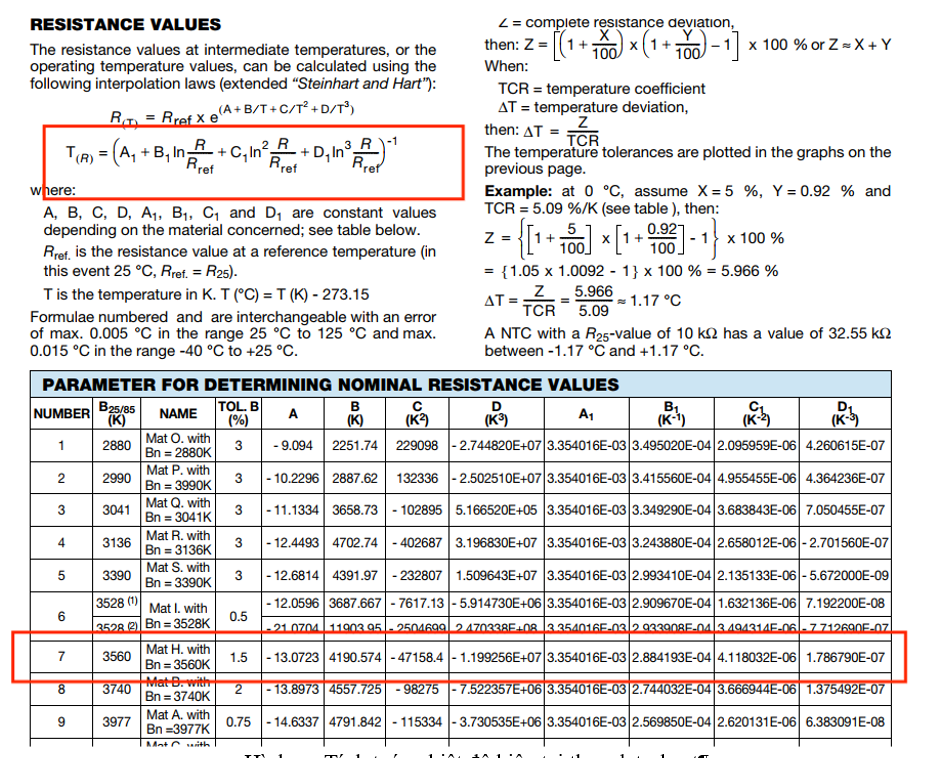
\includegraphics[width=0.9\linewidth]{my-chapters/my-images/Circuit_sim/CIRCUIT_pre_check_NTC}
	\caption{Tính toán nhiệt độ hiện tại theo datasheet.}
	\label{fig:circuitprecheckntc}
\end{figure}

\begin{figure}[H]
	\centering
	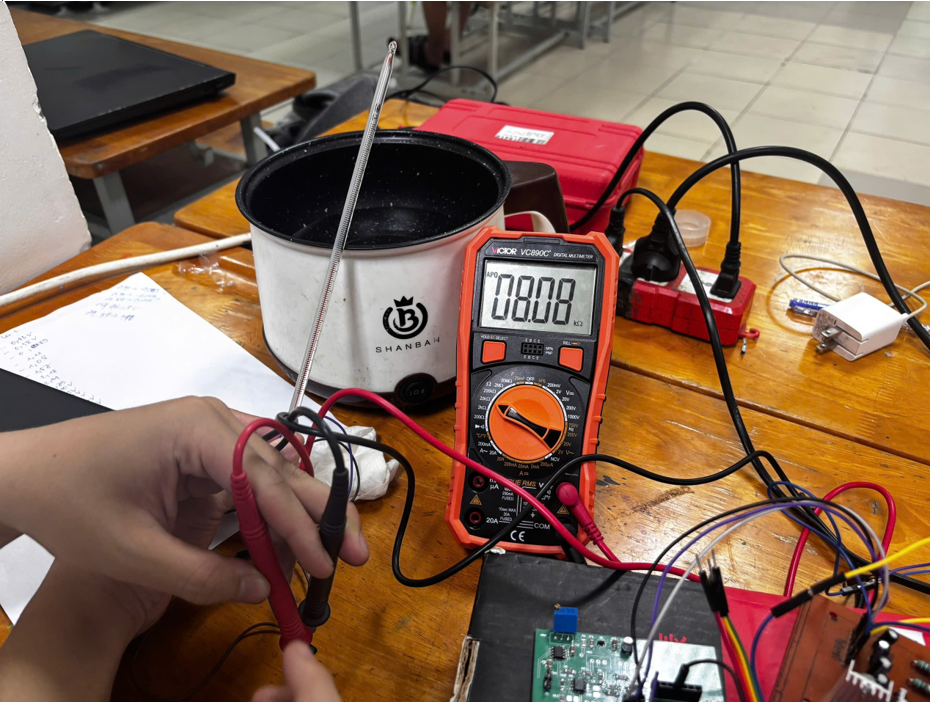
\includegraphics[width=0.8\linewidth]{my-chapters/my-images/Circuit_sim/CIRCUIT_pre_check_NTC_Vol}
	\caption{Kết quả đo điện trở ban đầu của NTC.}
	\label{fig:circuitprecheckntcvol}
\end{figure}

\begin{figure}[H]
	\centering
	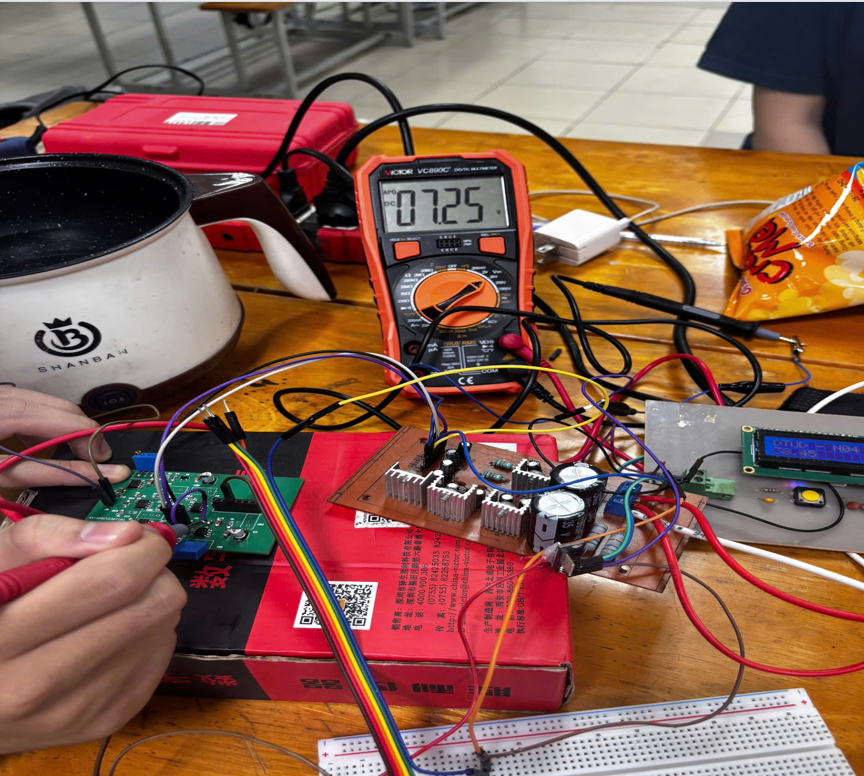
\includegraphics[width=0.8\linewidth]{my-chapters/my-images/Circuit_sim/CIRCUIT_pre_check_NTC_After_Vol}
	\caption{Tinh chỉnh điện áp từ $8\textsf{V}$ xuống $7.25\textsf{V}$.}
	\label{fig:circuitprecheckntcaftervol}
\end{figure}

Sau đó nhóm tiến hành khảo sát nhiệt độ và được kết quả thực nghiệm (video khảo sát : \href{https://youtu.be/sqnxJhxf1RI}{thislink})

%\begin{table}[H]
%	\centering
%	\caption{Kết quả thực nghiệm khảo sát nhiệt độ và điện áp}
%	\vspace{0.2cm}
%	\begin{tabular}{|c|c|}
%		\hline
%		\textbf{Nhiệt độ} & \textbf{Điện áp (V)} \\
%		\hline
%		15$^\circ$C & -0.12 \\
%		\hline
%		20$^\circ$C & 0.08 \\
%		\hline
%		25$^\circ$C & 0.39 \\
%		\hline
%		30$^\circ$C & 0.76 \\
%		\hline
%		35$^\circ$C & 1.13 \\
%		\hline
%		40$^\circ$C & 1.53 \\
%		\hline
%		45$^\circ$C & 2.08 \\
%		\hline
%		50$^\circ$C & 2.35 \\
%		\hline
%		55$^\circ$C & 2.69 \\
%		\hline
%		60$^\circ$C & 3.82 \\
%		\hline
%		65$^\circ$C & 5.92 \\
%		\hline
%		70$^\circ$C & 5.92 \\
%		\hline
%		75$^\circ$C & 5.92 \\
%		\hline
%		80$^\circ$C & 5.92 \\
%		\hline
%	\end{tabular}
%\end{table}

\begin{figure}[H]
	\centering
	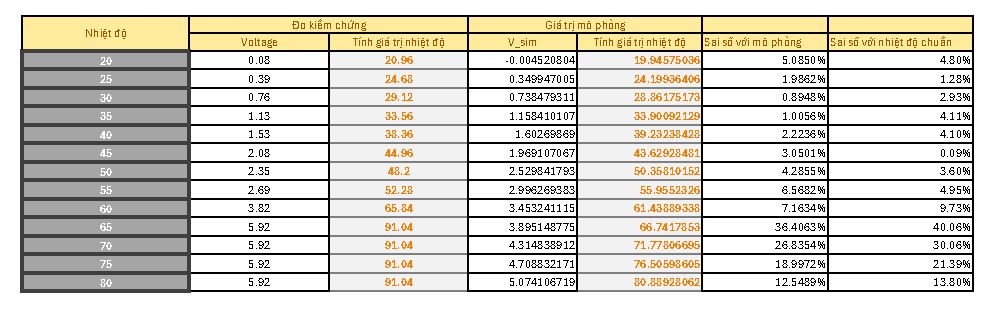
\includegraphics[width=\linewidth]{./my-ref/saiso_dodac.pdf}
	\caption{Kết quả thực nghiệm khảo sát nhiệt độ và điện áp.}
\end{figure}

\begin{itemize}
	\item \textbf{Nhận xét:} Từ nhiệt độ $20 \rightarrow 80 ^{o}C$ mach dao động từ 0.08 V đến 5.92V và từ 65 độ trở đi hầu như điện áp luôn bị ghim ở khoản $5.92\textsf{V}$.
\end{itemize}

Để biết được lý do việt từ 65 độ trở đi điện áp luôn bị ghim ở 5.92 V nhóm tiến hành khảo sát điện áp ngõ vào của INA128 vào ngõ ra ( video khảo sát \href{https://youtu.be/FasT7o_97dM}{thislink})

Từ video khảo sát ta có thấy từ khoảng 65 độ trở đi sự thay đổi điện áp ngõ vào gần như chỉ khoảng từ vài mV điều này khiến cho vôn kế không thể thay đổi nên điện áp luôn hiện thị $5.92$ đến $5.94\textsf{V}$.

\subsubsection{Kết luận}

Về cơ bản, mạch đã hoạt động đúng theo yêu cầu thiết kế ban đầu: khi nhiệt độ môi trường tăng, điện áp ngõ ra cũng tăng tương ứng. Tuy nhiên, kết quả thu được vẫn tồn tại sự sai số khá lớn so với tính toán lý thuyết. Những nguyên nhân chính dẫn đến sự sai lệch này có thể xuất phát từ dung sai của linh kiện, phương pháp đo đạc thủ công chưa đồng bộ, hoặc do ảnh hưởng của nhiễu từ môi trường xung quanh.
Bên cạnh vấn đề về sai số, trong quá trình thực hiện đề tài nhóm cũng đã đối mặt với không ít khó khăn. Việc tính toán để tuyến tính hóa đặc tuyến của cảm biến NTC cũng như cân chỉnh mạch sao cho hoạt động ổn định đòi hỏi nhiều thời gian thử nghiệm và khắc phục lỗi.

Mặc dù vậy, kết quả đạt được ngày hôm nay là minh chứng rõ ràng cho sự nỗ lực nghiên cứu và tinh thần làm việc nghiêm túc của tập thể nhóm.  Đề tài này không chỉ giúp nhóm hoàn thành mục tiêu học tập mà còn mang lại những kinh nghiệm thực tiễn quý báu .
